%NOTE TO SELF:
% Add flowchart of method (and overview)
% Merge section on simulation model and areas of study?
% Merge section on Simulation evaluation and data analysis?
% You can maybe divide the method into two parts: a Hindcast section and a Forecast section

\section{Overview of Methodology}

	\begin{figure}	
		\centering
		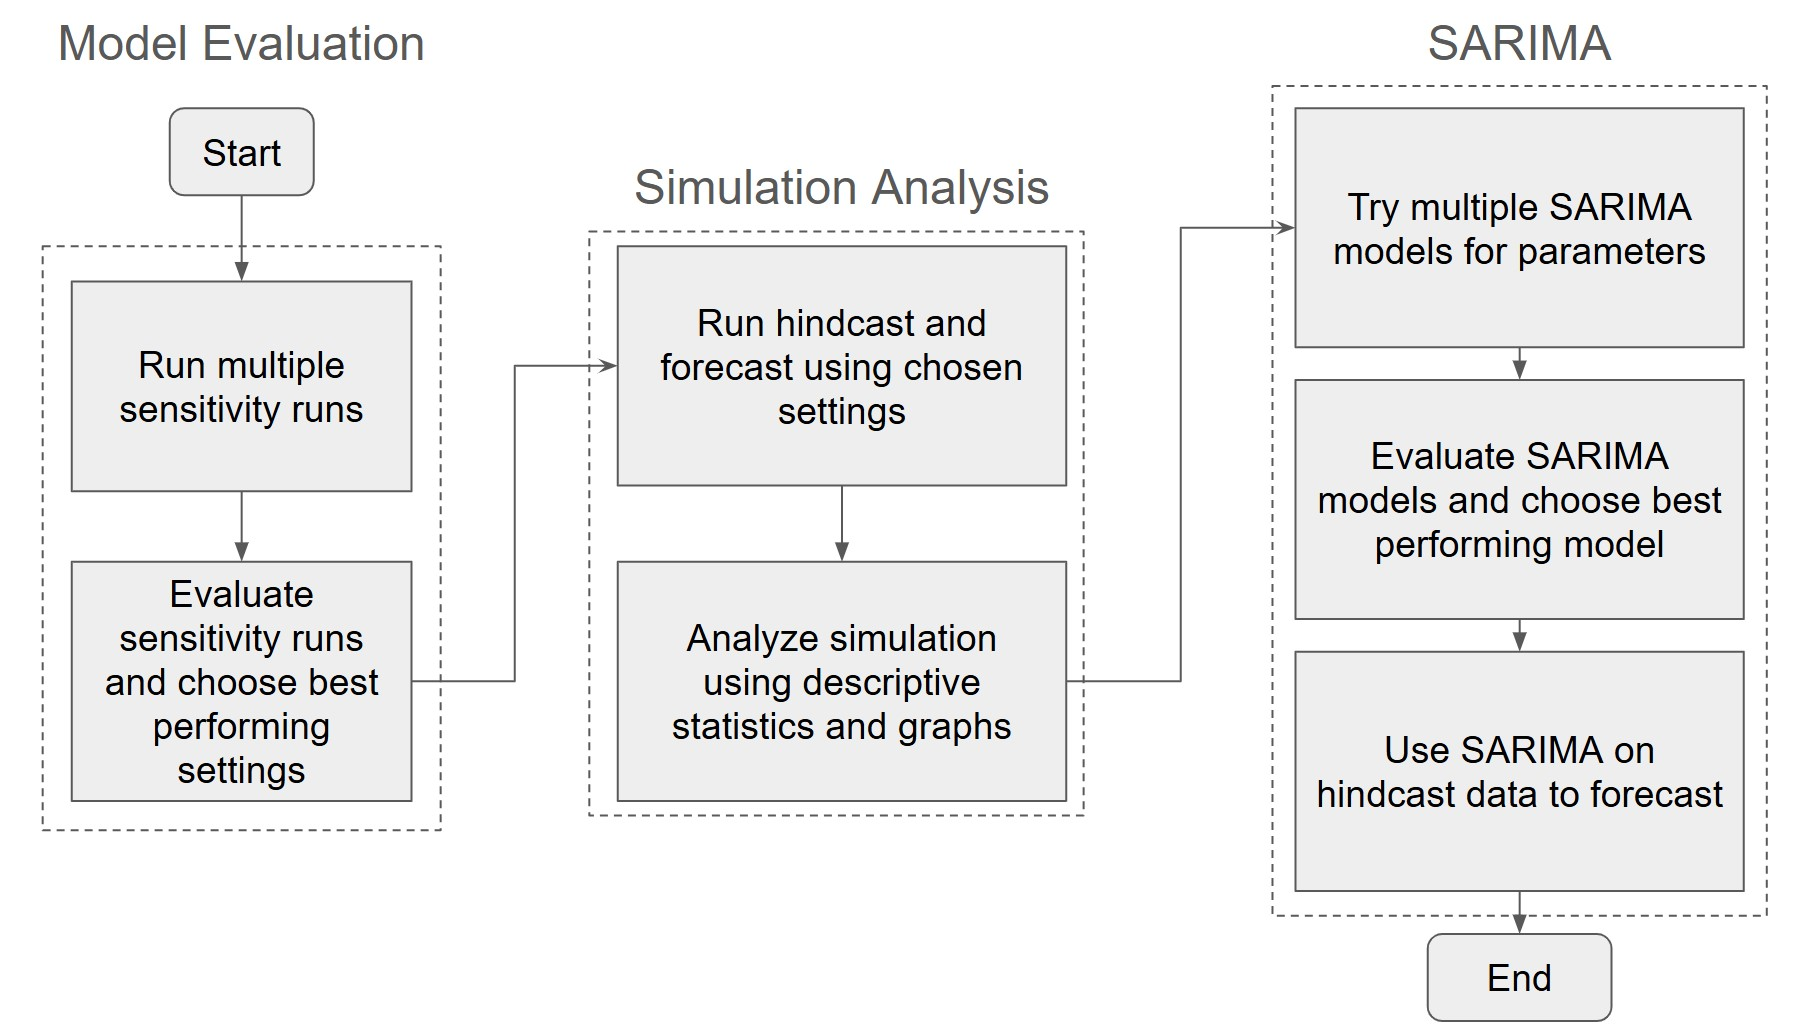
\includegraphics[width = \textwidth]{schematic-methodology}		
		\caption{
			A schematic of the methodology used in this study.
		}
		\label{fig:schematic-method}
	\end{figure}	
		
	Multiple sensitivity simulations were first performed in order to see which settings are most accurate for forecasting.
	The output of the sensitivity simulations were compared to observed weather data in order to assess their accuracy.
	Then, both hindcast and forecast simulations were conducted using the settings from the model evaluation.
	Analysis of this simulation was done to observe the trends in near-surface air temperature.
	Lastly, a SARIMA model is applied to the hindcast data.
	Multiple SARIMA parameters were evaluated, and the best performing parameters were chosen to forecast the near-surface air temperature.
	A flowchart of the methodology is provided in Figure \ref{fig:schematic-method}.

%	This study will be conducted over Metro Manila, Philippines.
%	Metro Manila, formally known as the National Capital Region, is the capital region of the Philippines.
%	The region has a land area of 636 square kilometers	and has a population of 13 million people (\cite{PSA2021}).
%	It is composed of one municipality: Pateros, and sixteen cities:
%		Caloocan,
%		Las Pinas,
%		Makati,
%		Malabon,
%		Mandaluyong,
%		Manila,
%		Marikina,
%		Muntinlupa,
%		Navotas,
%		Paranaque,
%		Pasay,
%		Pasig,
%		Quezon City,
%		San Juan,
%		Taguig, and
%		Valenzuela.
%	A map of Metro Manila is seen in Figure \ref{fig:map-of-metro-manila}.
	
	\begin{figure}
		\centering
		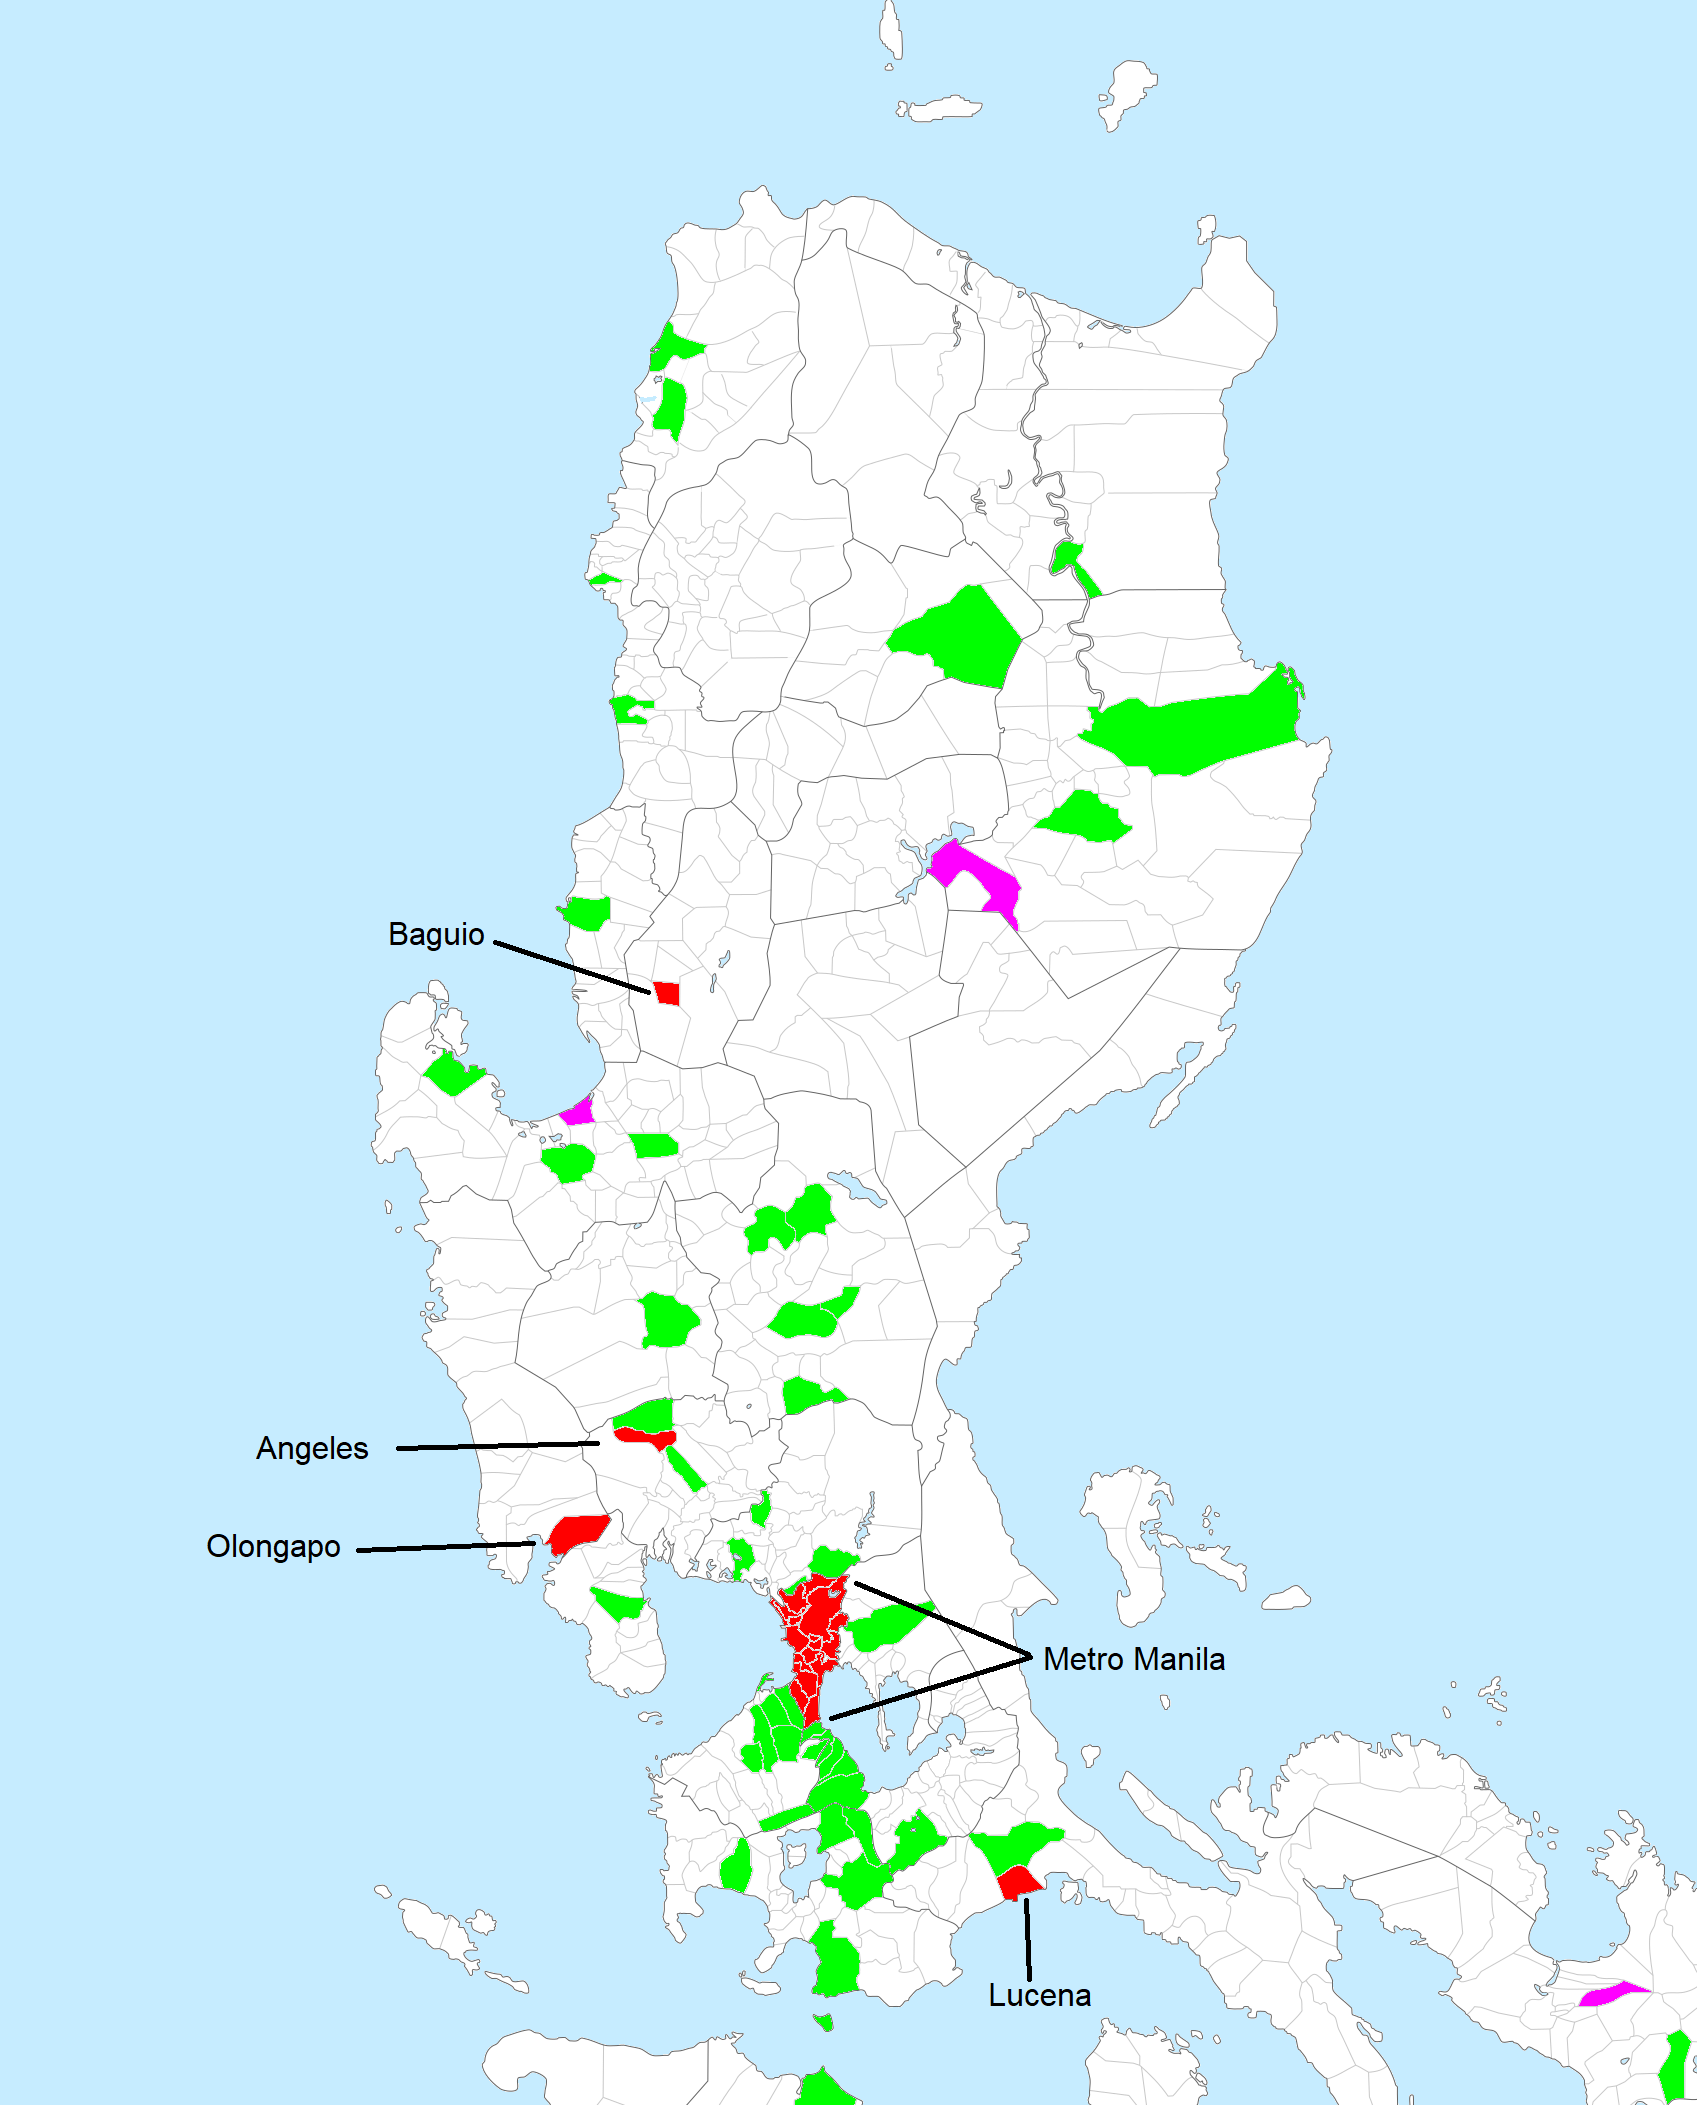
\includegraphics[width=13cm]{map-of-luzon}
		\caption{
			A partial map of Luzon showing its cities and municipalities.
			Highly urbanized cities are highlighted in red,
				Independent Component cities in purple,
				Component cities in green, and
				Municipalities in white.
			Adapted from user Sanglahi86, 	
				\href{https://creativecommons.org/licenses/by-sa/4.0}{CC BY-SA 4.0},
				via \href{https://commons.wikimedia.org/wiki/File:Cities_and_municipalities_of_the_Philippines.png}{Wikimedia Commons}.
		}
		\label{fig:map-of-metro-manila}
	\end{figure}	
		
\section{Simulation Model}
	This study used the latest version of the Regional Climate Model, RegCM5, which is described in detail by \textcite{Giorgi2023}.
	RegCM5 is a limited area model for long-term regional climate simulation.
	It is developed by the Abdus Salam International Centre for Theoretical Physics.
	The previous version, RegCM4, was released in 2012 (\cite{Giorgi2012}).
	
	\begin{table}	
		\caption{Configuration of the RegCM5 physics schemes.}
		\label{tab:physics-schemes}
		\centering
		%\begin{tabular}{p{2 in} p{2.75 in}}
		\begin{tabular}{l l}
			\hline \hline
			Physics scheme & Configuration\\
			\hline
			Atmospheric radiation & Radiation scheme from \textcite{Kiehl1996} \\
			Land surface model & Community Land Model 4.5 (\cite{Oleson2013})\\
			Planetary boundary layer & Based on \textcite{Holtslag1990}\\
			Cumulus convection & Based on \textcite{Emanuel1991}\\
			Resolvable scale precipitation & Subgrid explicit moisture scheme (\cite{Pal2000})\\
			\hline
		\end{tabular}		
	\end{table}
	
	Table \ref{tab:physics-schemes} shows the physics schemes used in the study.
	These schemes, with the exception of the land surface model, was used because they are the default schemes. 
	For the land surface model, the Community Land Model version 4.5 was chosen over the default, the Biosphere-Atmosphere Transfer Scheme. 
	Compared to the simpler default land surface scheme, the Community Land Model provides a more comprehensive description for land surfaces and contains a scheme for urban canopy simulation.
	
	\subsection{Domain of Study}
		Luzon is the largest island in the Philippines.
		This study analyzed six cities situated in Luzon:
		Angeles,
		Baguio,
		Manila,
		Olongapo,
		Pasay,
		and
		Quezon.
		These cities were chosen because they are all highly-urbanized cities with weather data available from the Integrated Surface Dataset.
		A partial map of Luzon can be seen in Figure \ref{fig:map-of-metro-manila}.
		
		The domain of the simulation can be seen in Figure \ref{fig:domain-luzon}.
		The center is placed at a longitude of 121◦ (centered on Metro Manila) and a latitude of 15.5◦ (1◦ above Metro Manila).
		This domain was chosen such that all of the chosen cities are roughly centered on the domain (i.e. away from the domain boundaries in order to avoid boundary issues).
		Vertical levels are configured to have 40 grid cells, with the top level corresponding to a pressure of \qty{50}{hPa}.
		This domain is used for both the hindcast and the forecast.
		
		\begin{figure}
			\centering
			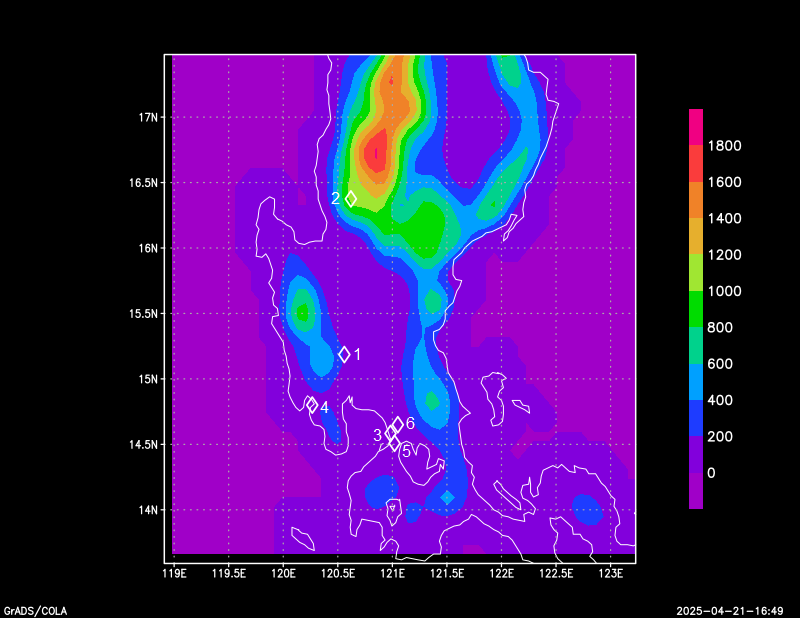
\includegraphics{domain-luzon.png}
			\caption{
				The domain of the run, Luzon.
				Color represents elevation in meters.
				Places marked with a diamond are the selected cities to be studied (listed in Table \ref{tab:isd-stations}).
			}
			\label{fig:domain-luzon}
		\end{figure}	
		
	
\section{Hindcast Simulations}
	The first part of this study conducted hindcast simulations.
	First, 
	Then, the chosen simulation was run again to simulate more years, and then analyzed.
	
\section{Model Evaluation}
	This study first conducted sensitivity runs in order to determine which settings to use in order to get accurate results.
	Sensitivity simulations of Luzon were ran over a four-year period, starting from 2014, January 2 up to 2018, January 1.
	The first year was considered as spin-up time and was ignored.
	Thus, only the three-year simulation period from 2015, January 1 to 2018, January 1 was considered for the data analysis.
	The simulation is set to output the results every 3 hours.
	Four sensitivity simulations were run:
	The first two simulations used the EIN15 dataset, a global
	atmospheric reanalysis by the European Centre for
	Medium-Range Weather Forecasts and described in \textcite{Dee2011}, for the initial conditions and boundary
	conditions (ICBC).
	The first run used a horizontal resolution of 16 km (28 by 30 grid cells), while the second run had double the resolution (8 km, 59 by 56 grid cells).
	The last two runs used the CNRM-CM5, a general circulation model as described in \textcite{Voldoire2012}, for the ICBC.
	As with the EIN15 runs, one was run with double the resolution of the other.
	A summary of the simulations run is in Table \ref{tab:summary-sensitivity-runs}.
	\begin{table}[]
		\caption{The ICBC and horizontal resolutions used for each of the four sensitivity simulations in this study.}
		\label{tab:summary-sensitivity-runs}
		\centering
		\begin{tabular}{ll}
			\hline \hline 
			ICBC Dataset & Horizontal resolution \\
			\hline
			EIN15 & 16 km (28 $\times$ 30 grid cells) \\
			EIN15 & 8 km (59 $\times$ 56 grid cells) \\
			CNRM-CM5 & 16 km (28 $\times$ 30 grid cells) \\
			CNRM-CM5 & 16 km (59 $\times$ 56 grid cells) \\
			\hline
		\end{tabular}
	\end{table}
	
	To determine the performance of the sensitivity simulation, an evaluation was performed. The evaluation procedure was adapted from \textcite{Bilang2022}.
	The results of the simulation was compared to real data from the Integrated Surface Database (ISD).
	The ISD is maintained by the United States National Oceanic and Atmospheric Administration, and is readily available on their website 
		(\url{https://www.ncei.noaa.gov/products/land-based-station/integrated-surface-database}).
	Data points missing from the data set were handled by replacing them with the mean of the data.
	The areas of study as well as their corresponding stations to be used in the evaluation are listed in Table \ref{tab:isd-stations}.

	\begin{table}	
		\caption{Areas of study and their corresponding stations in the Integrated Surface Dataset (ISD).}
		\label{tab:isd-stations}
		\centering
		\begin{tabular}{lll}
			\hline \hline
			& Area of Study             & ISD Station Name                       \\
			\hline
			1 & Angeles, Pampanga         & Clark International Airport        \\
			2 & Baguio, Benguet           & Baguio                             \\
			3 & Manila, Metro Manila      & Manila                             \\
			4 & Olongapo, Zambales        & Cubi Point                         \\
			5 & Pasay, Metro Manila      & Ninoy Aquino International Airport \\
			6 & Quezon City, Metro Manila & Science Garden \\                   
			\hline
		\end{tabular}	
	\end{table}

	Four performance statistics were computed using equations \ref{eq:mean-bias} to \ref{eq:y-bar},
		where $y_i$ is the modeled value, $y_{i,\text{obs}}$ is the observed value, and $N$ is the number of data points (\cite{Bilang2022}).
	The mean bias (MB) is a measure of the model to overestimate or underestimate a variable (\cite{Carbonell2013}), and is calculated by
	\begin{equation}
		\text{MB} =
			\frac{1}{N}
			\sum_{i=1}^{N}
			(y_i - y_{i,\text{obs}}).
			\label{eq:mean-bias}
	\end{equation}
	The mean absolute error (MAE) is used to measure the closeness of the modeled and observed values (\cite{Arasa2016}).
	It is calculated by
	\begin{equation}
		\text{MAE} =
			\frac{1}{N}
			\sum_{i=1}^{N} 
			|y_i - y_{i,\text{obs}}|. \label{eq:mean-absolute-error}
	\end{equation}
	The root mean square error (RMSE) is similar to the MAE but more sensitive to large errors due to the squared term (\cite{Carbonell2013}).
	It is calculated by
	\begin{equation}
		\text{RMSE} =
		\sqrt{
			\frac{
				\sum_{i=1}^{N}
				(y_i - y_{i,\text{obs}}) ^ 2
			}{N}
		}.
		\label{eq:root-mean-square-error}
	\end{equation}
	Lastly, the index of agreement (IOA), introduced by \textcite{Willmott1980}, shows how an error-free model predicts a variable.
	The index ranges between \num{0} and \num{1},
		with a value of \num{0} meaning no agreement between the model and observed data,
		and a value of \num{1} meaning a perfect match. 
	It is computed as
	\begin{equation}
		\text{IOA} =
			1 - 
			\frac{
				\sum_{i=1}^{N}
				(y_i - y_{i,\text{obs}}) ^ 2
			}{
				\sum_{i=1}^{N} (
					|y_i - \bar{y}| +
					|y_{i,\text{obs}} - \bar{y}|
				)^2
			},
			\label{eq:index-of-agreement}
	\end{equation}
	where
	\begin{equation}
		\bar{y} = 
			\frac{1}{N}
			\sum_{i=1}^{N} y_{i,\text{obs}}.
			\label{eq:y-bar}
	\end{equation}
	Before computing the statistics, the model values were first rounded to the nearest tenth in order to match the accuracy of the observed values from the ISD.
	The threshold for these values to determine if the model is performing well are given in Table \ref{tab:performance-statistics-threshold}, as adapted from \textcite{Bilang2022}.

	\begin{table}	
		\caption{Recommended values of statistical tests for near-surface air temperature.}
		\label{tab:performance-statistics-threshold}
		\centering
		\begin{tabular}{l l}
			\hline \hline
			Statistical parameter & Criteria\\
			\hline
			MB & $\leq \pm \qty{2.0}{\degreeCelsius}$ \\
			RMSE & $\leq \qty{3.5}{\degreeCelsius}$\\
			MAE & $\leq \pm \qty{2.0}{\degreeCelsius}$\\
			IOA	& $\geq \num{0.8}$\\
			\hline
		\end{tabular}		
	\end{table}

\section{Hindcast and Forecast}
		After the best-performing parameters were chosen, the model was run again to simulate more years.
		The simulation was run for another year until 2018, December 31.
		Then another simulation was run from 2012, January 1 to 2014, December 31,
			with the year 2012 considered as spin-up time.
		The new data is combined with data from the model evaluation data to give hindcast data from 2013 to 2018.
		
		Then, a forecast was also simulated.
		The simulation started on 2026, January 2 and ended on 2031, December 31.
		The year 2026 is considered as spin-up time and was ignored.
		Thus, the five-year simulation period from 2027, January 1 to 2032, January 1 was considered for analysis.
		
		For the analyses, yearly and monthly means, minimums, and maximums were calculated and graphed, and the mean diurnal temperature of the hottest year per season was also calculated and graphed.
		For the urban heat island intensity, temperature from the cities were compared to nearby rural areas. For Pasay, Manila, and Quezon, the rural area was Naic, Cavite. For Angeles, it was Capas, Tarlac. For Baguio, it was Itogon, Benguet.
		Urban heat island intensity was calculated using Equation \ref{eq:uhii}.
		
\section{SARIMA}
	A seasonal autoregressive integrated moving average model (SARIMA) was trained on the hindcast data.
	First, the hindcast data was resampled to monthly mean data for the purposes of training the SARIMA model.
	The years 2013 to 2016 of the hindcast data are used for training the model, while the years 2017 to 2018 are used for testing the data.
	The autocorrelation plots were generated in order to find possible values for parameters in the SARIMA model.
	Various models with different SARIMA parameters are tested.
	For each model, the MB, MAE, and RMSE (Equations \ref{eq:mean-bias} to \ref{eq:root-mean-square-error}) was calculated.
	In addition, the Akaike information criterion (AIC) was calculated.
	The AIC is a measure of the quality of a given model compared to other models, and is used in model selection.
	It is given by the equation
	\begin{equation}
		\operatorname{AIC} = n \ln \left( 
			\frac{\operatorname{RSS}}{n} 
		\right) + 2K,
		\label{eq:akaike-information-criterion}
	\end{equation}
	where $n$ is the number of data points,
		$\operatorname{RSS}$ is the residual sums of squares,
		and
		$K$ is the number of parameters in the model
		(\cite{Chen2018}).
	The model with the lowest AIC was chosen as the model to forecast with.
	After choosing the model, it was retrained using the entire hindcast data and then forecasted up to the year 2030.